\chapter{Material e Métodos}
Neste capítulo serão descritas as fases de especificação e projeto do sistema. As
outras fases da engenharia de software serão desenvolvidas e apresentadas na
defesa da monografia.

\section{Engenharia de Software}

Engenharia de Software pode ser definida como:
\begin{citacao}[english]
1. the systematic application of scientific and technological knowledge, methods, and experience to the design,
implementation, testing, and documentation of software [...]  2. the application
of a systematic, disciplined, quantifiable approach to the development, operation,
and maintenance of software; that is, the application of engineering to software \cite{IEEE2010}.
\end{citacao}

\begin{figure}[!b]
  \centering
  \caption{Engenharia de Software - uma tecnologia em camadas}
  
\includegraphics[scale=0.33]{imagens/desenv_engsoft2}
  \label{fig:desen_engsoft}
  \fonte{\cite{Pressman2009}}
\end{figure}

A engenharia de software deve ter foco na qualidade, que apoia as outras camadas
dessa tecnologia, que são as camadas de processo, métodos e ferramentas \autoref{fig:desen_engsoft}.
A camada de processo define um conjunto de atividades ou um arcabouço que tem
como finalidade garantir a efetiva utilização da tecnologia engenharia de software, que dessa forma
leva à produção de um software. Os detalhes de como fazer o software pertencem
a camada de métodos. Os métodos da engenharia de software incluem tarefas de planejamento
e estimativa de software, análise de requisitos, modelagem de projeto, codificação,
testes e manutenção. As ferramentas de engenharia de software auxiliam as camadas de
processo e métodos, com ferramentas automatizadas, que por sua vez, quando integradas,
é estabelecido um suporte ao desenvolvimento de software chamado CASE -
\textit{Computer Aided Software Engineering} \cite{Pressman2009, Sommerville2006}.

Entre o conjunto de atividades definidas pela camada de processo, quatro são
fundamentais, a saber, especificação de software, projeto e implementação de
software, validação de software e evolução de software. Especificação de software
ou engenharia de requisitos é uma fase importante e crítica do processo de engenharia
de software. Importante porque é uma análise de requisitos bem feita que possibilitará
atendar as demandas dos usuários. Crítica porque um sistema mal especificado, pode até ser
bem projetado e construído, mas não vai atender as necessidades dos usuários.
Em seguida, na fase de projeto e implementação os requisitos são projetados e programados,
tendo como resultado um sistema executável. Depois, o software deve ser verificado
para mostrar que atende às demandas dos usuários (validação do software). Finalmente,
na fase de evolução de software, o mesmo é modificado devido às mudanças
de requisitos e às necessidades dos usuários.

\subsection{Especificação do Sistema}
Nessa primeira etapa do projeto, foi utilizada a ferramenta \textit{Astah Community} \cite{astah2016}
para a criação de documentação em linguaguem de modelagem unificada (UML). Os diagramas
de casos de uso UML são largamente utilizados para espeficificação de requisitos \cite{Sommerville2006}.
A \autoref{fig:usecases} exemplifica os casos de uso do sistema, fornecendo uma
visão geral do mesmo.

\begin{figure}[!htb]
  \centering
  \caption{Diagrama de Caso de Uso: Visão geral do sistema}
  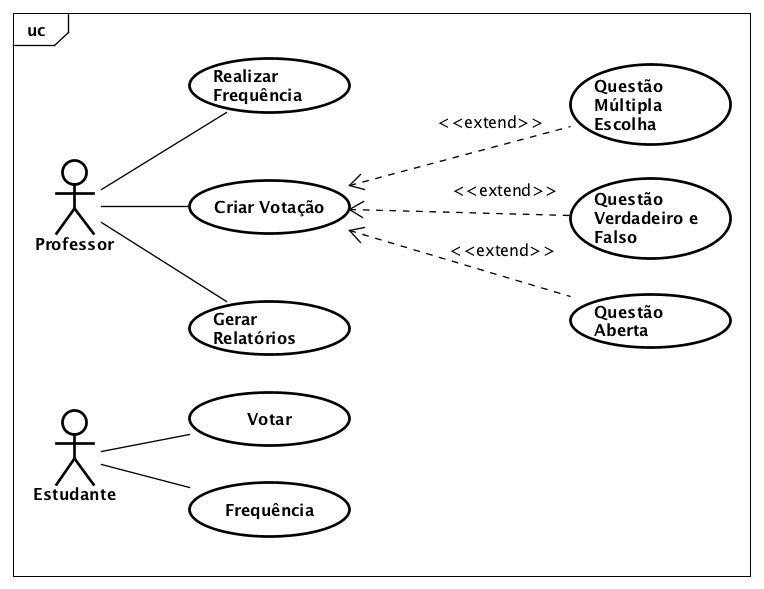
\includegraphics[width=.75\textwidth]{imagens/casodeuso}
  \fonte{Elaborado pelo autor}
  \label{fig:usecases}
\end{figure}

\subsection{Projeto e Implementação}
O diagrama de implantação UML ou \textit{deployment diagram} mostra o \textit{hardware}
do sistema ou elementos de processamento, os componentes de software instalados
no \textit{hardware} e o \textit{middleware} usado para conectar os diferentes
nós do sistema \cite{Pressman2009}. A \autoref{fig:deployment_diagram} mostra
o diagrama de implação do sistema que será desenvolvido. É possível observar
uma solução simples, mas que faz uso de soluções \textit{open-source} e de
qualidade reconhecida como será descrito a seguir.

\subsubsection{Plataforma}


\begin{figure}[!htb]
  \centering
  \caption{Diagrama de Implantação do sistema}
  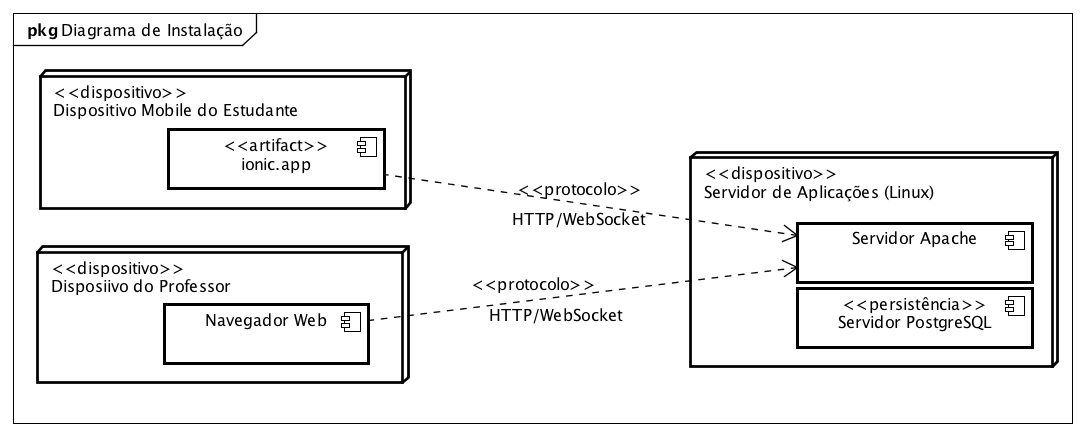
\includegraphics[width=1\textwidth]{imagens/deployment_diagram}
  \fonte{Elaborado pelo autor}
  \label{fig:deployment_diagram}
\end{figure}
